\documentclass[sigconf]{acmart}
\pagestyle{plain}
\usepackage{amsthm}

% Remove headers and footers
\pagestyle{plain}
% Set up two-column layout
\usepackage{geometry}
\geometry{twocolumn}
\usepackage{hyperref}
\def\sectionautorefname{Section} % needs to be capitalized according to LNCS guidelines
\def\subsectionautorefname{Subsection} % needs to be capitalized according to LNCS guidelines
% \usepackage[htt]{hyphenat}
\usepackage{subcaption}
\usepackage{amsmath,amsthm}
\usepackage{nimbusmononarrow}
\usepackage{MnSymbol}
\usepackage{algorithm}
\usepackage{algpseudocode}
\usepackage[utf8]{inputenc}
\usepackage{graphicx}
\usepackage[utf8]{inputenc}
\usepackage[english]{babel}
\settopmatter{printacmref=false}
\renewcommand\footnotetextcopyrightpermission[1]{}
\newcommand*{\defcon}{\ensuremath{\mathrel{\medvert\mskip-5.7mu\clipbox{1 0 0 0}{$\sim$}}}}
\newcommand*{\defent}{\ensuremath{\mathrel{\medvert\mskip-5.7mu\clipbox{1 0 0 0}{$\approx$}}}}
\newcommand*{\satisfy}{\ensuremath{\mathrel{\medvert\mskip-7mu\clipbox{1 0 0 0}{$\equiv$}}}}

% _______________
% Aux 
% _______________
\newcommand{\underlinesymbol}[1]{\underline{\vphantom{y}#1}}
\newcommand{\st}{\text{ s.t. }}
\newcommand{\wrt}{\text{w.r.t }}

% _______________
% General Defeasible Stuff
% _______________
\newcommand{\twiddle}{\mathrel|\joinrel\sim}                        % Twiddle
\newcommand{\ntwiddle}{\mathrel|\joinrel\not\sim}                   % Negation of twiddle

% _______________
% FCA 
% _______________
\newcommand{\K}{\mathbb{K}}                                         % K
\newcommand{\GMI} {(G,M,I)}
\newcommand{\FC}{\mathbb{K} = \GMI}                                 % Formal Context
\newcommand{\BK}{\mathfrak{B}\GMI}                                  % Set of all concepts
\newcommand{\CL}{\underlinesymbol{\mathfrak{B}}\GMI}
\newcommand{\minO}[1]{\underlinesymbol{#1}'}                        % single minimisation
\newcommand{\dminO}[1]{(\minO{#1})'}                                % double minimisation 

\newcommand{\ccbM}{\cellcolor[HTML]{b6bfdb}}
\newcommand{\ccbS}{\cellcolor[HTML]{b6dbb7}}
\newcommand{\ccr}{\cellcolor{red}}
\newcommand{\ccb}{\cellcolor{blue}}

% \title{Developing Non-monotonicity in Formal Concept Analysis}
\title{Rational Concept Analysis}

\author{Lucas Carr}
\affiliation{
  \department{Department of Computer Science}
  \institution{University of Cape Town}
}
\email{crrluc003@myuct.ac.za}
%
\begin{document}

\maketitle
\section{Introduction}
\label{section: introduction}

Formal concept analysis (FCA) provides a framework, grounded in lattice theory, for mathematically reasoning about \textit{formal concepts} and their hierarchies \cite{ganter1999formal,ganter2016conceptual,rudolph2007relational}. The matter of \textit{concepts} has largely been of Philosophical concern: the notion of a concept as the dualism between \textit{intension} and \textit{extension} has foundations in Aristotle's \textit{Organon} and, much later on, in the \textit{Logic of Port-Royal} \cite{rudolph2007relational,castonguay2012meaning}. In this view, the extension of a concept contains to those ``things'' that one might refer to as instances of the concept. Dually, intension describes the meaning, or \textit{sense}, of a concept.

Formal concept analysis---which adopts this view of concepts---introduces a \textit{formal context} as the structure of data. This is a triple consisting of a finite set of objects $G$, attributes $M$, and a binary relation, $I \subseteq G\times M$, which indicates that a particular object has a respective property \cite{ganter1999formal,ganter2016conceptual}. A \textit{formal concept} is a pair, made up of the formal concept extension and intension, respectively. The set of all concepts, when ordered by the \textit{sub/super-concept} relation, form the \textit{concept lattice} used for analysis.


Another important topic in FCA is the discovery of \textit{implications} that pertain to, or are \textit{respected} by, a context \cite{rudolph2007relational,ganter1999formal}. Implications are used to express correspondence between (sets) of attributes. The notion of a context \textit{respecting} an attribute implication is analogous to that of \textit{entailment} in classical logic \cite{ganter2016conceptual}. As such, \textit{respecting} describes a monotonic notion of consequence.

Discussion and work on non-monotonic propositional, first-order, and description logic is a well established topic in artificial intelligence, \cite{ferguson2003monotonicity,giordano2015semantic,kraus1990nonmonotonic,lehmann1994what,shoham1987nonmonotonic}. However, there does not appear to be any effort to introduce this expressivity to the attribute logic of FCA.

% That is not to say that increasing the expressivity of FCA's attribute logic would not be beneficial: association rules are a fairly blunt way of gaining some non-monotonicty in FCA. However, they acquire meaning through majority rule - where we would like something more precise.

% Applications of FCA: text mining, web mining, and ontology engineering

%
\section{Background}
\label{section: background}
\subsection{Formal Concept analysis}
\label{subsection: formal concept analysis}

\subsection{Classical Notions of Consequence}
\label{subsection: classical notions of consequence}

\subsection{Non-monotonic Consequence}
\label{subsection: non-monotonic consequence}
%
\section{Motivation for Research Area}
\label{section: motivation}

In practice, FCA has been implemented as a framework for information retrieval \cite{poelmans2012text}, program analysis, ontology engineering. Until very recently \cite{carr2024nonmonotonicextensionsformalconcept,ding2024defeasiblereasoningconcepts} there have been no attempts to lift the expressivity of FCA's attribute logic to a non-monotonic counterpart. To explicate why non-monotonicity would be desirable in the context of FCA, a toy example is provided.

When introducing younger children about the vertebrates it is often expressed that a defining feature of mammals is that they give birth to live young, and that reptiles lay eggs instead. Mammals and reptiles can be formalised as concepts \texttt{m} and \texttt{r}:
\small
\[
    \begin{aligned}
         & \texttt{m} \coloneq \texttt{\big(\{platypus,\ldots,horse\}, \{warm-blooded,\ldots,live young\}\big)}  \\
         & \texttt{r} \coloneq \texttt{\big(\{snake,\ldots,J-chameleon\}, \{cold-blooded,\ldots,lay eggs\}\big)}
    \end{aligned}
\]
\normalsize
There is, however, a problem with this construction. Namely, Jackson chameleons are reptiles that give birth to live young, and platypodes are mammals that lay eggs, and so they should not belong to these concepts. The classical FCA response to this issue might be that there should be two sub-concepts \texttt{m$_1$} and \texttt{m$_2$} of \texttt{m}. Then, \texttt{m$_1$} may specify those mammals which give birth to live young, and \texttt{m$_2$} those that lay eggs.

This argument forces the abandon the kind of reasoning that appears so central to our intuition. We do not think of mammals as being divided between those that give birth to live young and those that do not; moreover, there are likely several properties which cause similar rifts in conception. A more natural way of reasoning about this matter would be to think of Jackson chameleons as \textit{exceptional} mammals. \textit{Exceptionality} obviously suggests a counter notion of \textit{typicality}.

Another important concern is the use implications of a formal context to discover correspondence between attribute(s). As a reminder of \cref{definition: modelling an implication}, classical FCA implications are only valid in a formal context when they are respected by every object. Consequently, a context modelling birds and their attributes might find that, although most objects have wings and fly, there are exceptions (e.g., penguins, ostriches) which prevent \texttt{wings} $\rightarrow$ \texttt{fly} from being valid; and so we remain unenlightened about the relationship between these attributes. Once again, the classical framework does not handle exceptions well.

A method to describe implications which only partially hold in a formal context is desirable. \textit{Association rules} are an existing approach, and association rule mining in FCA has been discussed \cite{ganter2016conceptual,lakhal2005efficient}. Association rules, however, use \textit{confidence} and \textit{support} as a means of discovering relationships. These relationships then do not correspond to some describable pattern of reasoning—e.g., rational consequence relations—but are rather a flavour of `majority rules'.


%
\section{Research Questions \& Objectives}
\label{section: research objectives}

We now develop a more thorough framing of the problems discussed in \cref{section: motivation}, detailing the current view on what the correct questions are, and how we undertake finding their solutions.




% conceptual structuring of data, ontology engineering, software mining



% The aim of this work is to introduce KLM style non-monotonicity to the attribute logic underpinning FCA. Doing so creates two principle areas of interest. The first, and most obvious, concerns the notion of a \textit{non-monotonic implication} in FCA. Secondly, a corollary of introducing a ranking to a context is that it a provides expressivity to develop \textit{typical concepts}.

% Concerning non-monotonic implications, we begin our work by finding a translation from the weaker \textit{system P} to FCA. This system relies on being able to construct an ordering over the valuations of a knowledge base. We find that assuming a partial ordering over the set of objects in a formal context—implicitly providing a way to compare object intents—introduces a suitable structure for a semantic definition of preferential implications. \cref{definition: modelling an implication} can be altered to define a defeasible implication which is valid in a context iff the minimal objects in $A'$ are a subset of $B'$.


%
%
% \section{Non-monotonic FCA}
\label{section: non-monotonic fca}

\subsection{Defeasible Implications in FCA}
\label{subsection: defeasible implications in FCA}

\subsection{Rational Consequence}
\label{subsection: rational consequence}

\subsection{Typical Concepts}
\label{subsection: typical concepts}


%
% \section{Ethical, Professional, and Legal Issues}
\label{section: ethics}


%
\section{Project Plan}
\label{section: project plan}
%
\clearpage
%
\bibliography{refs.bib}
\bibliographystyle{ACM-Reference-Format}
%
\clearpage
%
\onecolumn
\section{Appendix}
% % Your table in single-column mode

\begin{figure}[h]
    \centering
    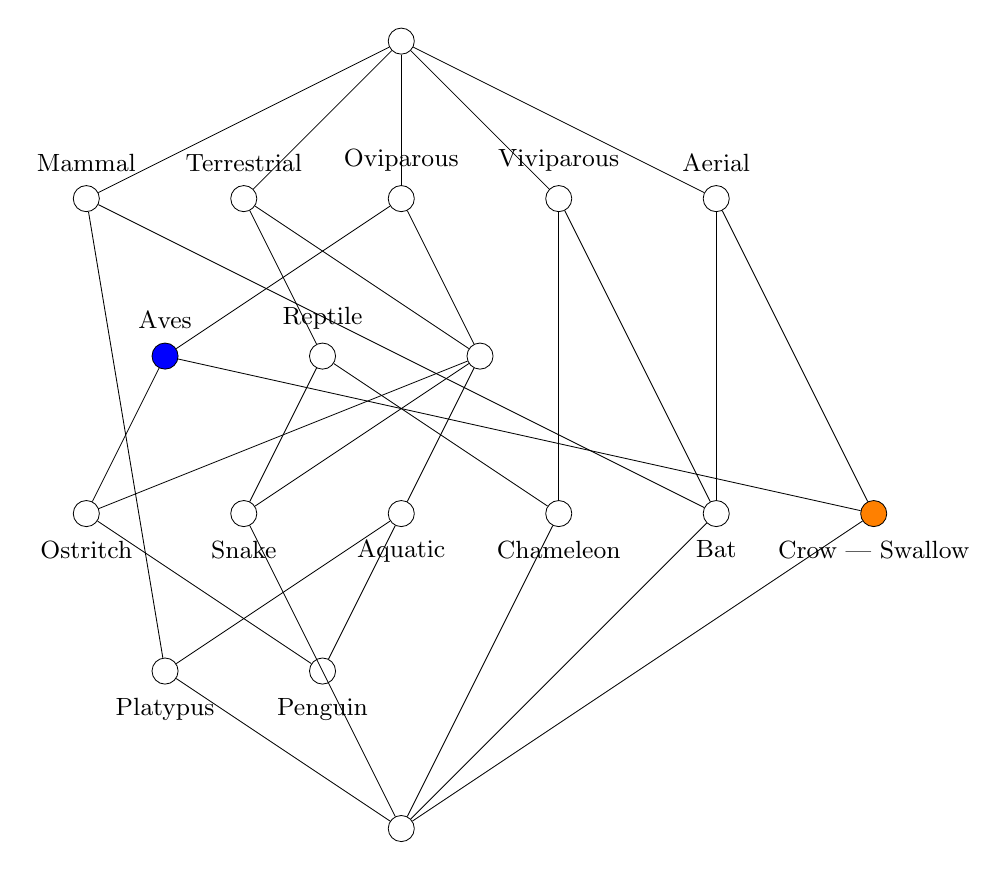
\begin{tikzpicture}[
            scale=1,
            concept/.style={circle, draw, line width=0.3pt, minimum size=0.2cm},
            label_above/.style={font=\small, above=0.05cm},
            label_below/.style={font=\small, below=0.05cm},
            line/.style={draw, line width=0.3pt}
        ]
        % Top node
        \node[concept] (root) at (0,8) {};

        % First level - characteristics
        \node[concept] (mammal) at (-4,6) {};
        \node[label_above] at (mammal.north) {Mammal};
        \node[concept] (terrestrial) at (-2,6) {};
        \node[label_above] at (terrestrial.north) {Terrestrial};
        \node[concept] (eggs) at (0,6) {};
        \node[label_above] at (eggs.north) {Oviparous};
        \node[concept] (young) at (2,6) {};
        \node[label_above] at (young.north) {Viviparous};
        \node[concept] (aerial) at (4,6) {};
        \node[label_above] at (aerial.north) {Aerial};

        % Middle level - classifications
        \node[concept,fill=blue] (aves) at (-3,4) {};
        \node[label_above] at (aves.north) {Aves};

        \node[concept] (mid_empty) at (1,4) {};

        \node[concept] (reptile) at (-1,4) {};
        \node[label_above] at (reptile.north) {Reptile};

        % Lower level
        \node[concept] (ostritch) at (-4,2) {};
        \node[label_below] at (ostritch.south) {Ostritch};
        \node[concept] (snake) at (-2,2) {};
        \node[label_below] at (snake.south) {Snake};
        \node[concept] (aquatic) at (0,2) {};
        \node[label_below] at (aquatic.south) {Aquatic};
        \node[concept] (chameleon) at (2,2) {};
        \node[label_below] at (chameleon.south) {Chameleon};
        \node[concept] (bat) at (4,2) {};
        \node[label_below] at (bat.south) {Bat};
        \node[concept,fill=orange] (crow) at (6,2) {};
        \node[label_below] at (crow.south) {Crow | Swallow};

        % Bottom level
        \node[concept] (platypus) at (-3,0) {};
        \node[label_below] at (platypus.south) {Platypus};
        \node[concept] (penguin) at (-1,0) {};
        \node[label_below] at (penguin.south) {Penguin};

        \node[concept] (bot) at (0,-2) {};

        \draw[line] (mammal) -- (root);
        \draw[line] (terrestrial) -- (root);
        \draw[line] (eggs) -- (root);
        \draw[line] (young) -- (root);
        \draw[line] (aerial) -- (root);

        \draw[line] (eggs) -- (aves);
        \draw[line] (eggs) -- (mid_empty);
        \draw[line] (terrestrial) -- (reptile);
        \draw[line] (terrestrial) -- (mid_empty);

        \draw[line] (mammal) -- (bat);
        \draw[line] (mammal) -- (platypus);

        \draw[line] (young) -- (bat);
        \draw[line] (young) -- (chameleon);

        \draw[line] (aerial) -- (bat);
        \draw[line] (aerial) -- (crow);

        \draw[line] (aves) -- (ostritch);
        \draw[line] (aves) -- (crow);

        \draw[line] (reptile) -- (snake);
        \draw[line] (reptile) -- (chameleon);

        \draw[line] (mid_empty) -- (snake);
        \draw[line] (mid_empty) -- (ostritch);
        \draw[line] (mid_empty) -- (aquatic);

        \draw[line] (crow) -- (bot);

        \draw[line] (ostritch) -- (penguin);

        \draw[line] (aquatic) -- (penguin);
        \draw[line] (aquatic) -- (platypus);

        \draw[line] (bat) -- (bot);

        \draw[line] (snake) -- (bot);

        \draw[line] (chameleon) -- (bot);

        \draw[line] (platypus) -- (bot);

    \end{tikzpicture}
    \caption{Concept lattice for the formal context in \cref{table: formal context}.}

    \label{figure: concept lattice}
\end{figure}

\begin{table}[h]
    \centering
    \begin{tabular}{rcccccccc}
                              & \texttt{Aves} & \texttt{Mammal} & \texttt{Reptile} & \texttt{Aerial} & \texttt{Aquatic} & \texttt{Terrestrial} & \texttt{Live Young} & \texttt{Eggs} \\
        \hline
        \texttt{Bat}          &               & $\times$        &                  & $\times$        &                  &                      & $\times$            &               \\
        \texttt{Crow}         & $\times$      &                 &                  & $\times$        &                  &                      &                     & $\times$      \\
        \texttt{Ostrich}      & $\times$      &                 &                  &                 &                  & $\times$             &                     & $\times$      \\
        \texttt{Penguin}      & $\times$      &                 &                  &                 & $\times$         & $\times$             &                     & $\times$      \\
        \texttt{Platypus}     &               & $\times$        &                  &                 & $\times$         & $\times$             &                     & $\times$      \\
        \texttt{Snake}        &               &                 & $\times$         &                 &                  & $\times$             &                     & $\times$      \\
        \texttt{Swallow}      & $\times$      &                 &                  & $\times$        &                  &                      &                     & $\times$      \\
        \texttt{J. Chameleon} &               &                 & $\times$         &                 &                  & $\times$             & $\times$            &               \\
    \end{tabular}
    \vspace{10pt}
    \caption{A formal context describing animals (objects) and some of their features (attributes)}
    \label{table: formal context}
\end{table}
\clearpage

% \twocolumn

% \begin{table}
% 	\centering
% 	\begin{tabular}{r|c|c|c|c|c|c|c|c|c|c}
% 		                   & \texttt{Aves} & \texttt{Mammal} & \texttt{Reptile} & \texttt{Aerial} & \texttt{Aquatic} & \texttt{Terrestrial} & \texttt{Migratory} & \texttt{Solitary} & \texttt{Carnivore} & \texttt{Eggs} \\
% 		\hline
% 		\texttt{Bat}       &               & $\times$        &                  & $\times$        &                  &                      &                    &                   & $\times$           &               \\
% 		\texttt{Crocodile} &               &                 & $\times$         &                 & $\times$         & $\times$             &                    &                   & $\times$           & $\times$      \\
% 		\texttt{Crow}      & $\times$      &                 &                  & $\times$        &                  &                      &                    &                   &                    & $\times$      \\
% 		\texttt{Hippo}     &               & $\times$        &                  &                 & $\times$         & $\times$             &                    & $\times$          &                    &               \\
% 		\texttt{Ostrich}   & $\times$      &                 &                  &                 &                  & $\times$             &                    & $\times$          &                    & $\times$      \\
% 		\texttt{Penguin}   & $\times$      &                 &                  &                 & $\times$         & $\times$             & $\times$           &                   & $\times$           & $\times$      \\
% 		\texttt{Platypus}  &               & $\times$        &                  &                 & $\times$         & $\times$             &                    & $\times$          & $\times$           & $\times$      \\
% 		\texttt{Snake}     &               &                 & $\times$         &                 &                  & $\times$             &                    & $\times$          & $\times$           & $\times$      \\
% 		\texttt{Swallow}   & $\times$      &                 &                  & $\times$        &                  &                      & $\times$           & $\times$          & $\times$           & $\times$      \\
% 		\texttt{Whale}     &               & $\times$        &                  &                 & $\times$         &                      & $\times$           & $\times$          & $\times$           &               \\
% 	\end{tabular}
% 	\caption{Cross-table of $\K$}
% 	\label{tab:formal-context}
% \end{table}


% \begin{algorithm}
% 	\caption{Computing the tolerance partition on objects $G$}
% 	\begin{algorithmic}[1]
% 		\Require A formal context, $\FC$;
% 		\Require A set of defeasible implications, $\Delta$;
% 		\Ensure A tolerance partition $(R_0, \ldots, R_n)$ on $G$;
% 		\State $P_0 \gets G$;
% 		\State $i \gets 0$;
% 		\State $\Delta \gets \text{Material} (\Delta)$;
% 		\While {$P_{i-1} \neq P_i}$
% 			\State $P_{i+1} \gets \{g \in P_i \mid \exists \delta \in \Delta  g' \st g'\not \models \delta \}$;
% 			\State $R_i \gets P_i \setminus P_{i+1}$;
% 			\State $\Delta_i \gets \{ (\alpha \rightarrow \beta) \in \Delta \mid \exists g \in P_i \st \alpha \subseteq g'\}$;
% 			\State $\Delta \gets \Delta \setminus \Delta_i$;
% 			\EndWhile
% 			\If {$P_{i-1} = \emptyset$}
% 			\State $n \gets i-1$;
% 			\Else
% 			\State $n \gets i$;
% 			\EndIf
% 			\State \Return $\big (R_0,\ldots, R_n \big)$;
% 	\end{algorithmic}
% \end{algorithm}

% To clarify some points on
% \begin{itemize}
% 	\item Line $3$: this step turns $\Delta$ into a set of material implications;
% 	\item Line $5$: this step puts into ranking $i+1$ every object which \textbf{does not} respect $\Delta$;
% 	\item Line $7$: this sets $\Delta_i$ to be the set of formulae in $\Delta$ which have their antecedent satisfied by an object in $P_i$ (implicitly all objects in $P_i$ satisfy all formulae in $\Delta$, but we only care about the ones which have their antecedent satisfied);
% 	\item We update $\Delta$ to be those formulae which are not yet ``dealt with''.
% \end{itemize}

% \begin{algorithm}
% 	\caption{Checking entailment}
% 	\begin{algorithmic}[1]
% 		\Require A formal context, $\FC$;
% 		\Require A set of defeasible implications, $\Delta$;
% 		\Ensure A tolerance partition $(R_0, \ldots, R_n)$ on $G$;
% 		\State $P_0 \gets G$;
% 		\State $i \gets 0$;
% 		\State $\Delta \gets \text{Material} (\Delta)$;
% 		\While {$P_{i-1} \neq P_i}$
% 			\State $P_{i+1} \gets \{g \in P_i \mid \exists \delta \in \Delta  g' \st \not \Vdash \delta \}$;
% 			\State $P_i \gets P_i \setminus P_{i+1}$;
% 			\State $\Delta_i \gets \{ (\alpha \rightarrow \beta) \in \Delta \mid \exists g \in P_i \st \alpha \subseteq g'\}$;
% 			\State $\Delta \gets \Delta \setminus \Delta_i$;
% 			\EndWhile
% 			\If {$P_{i-1} = \emptyset$}
% 			\State $n \gets i-1$;
% 			\Else
% 			\State $n \gets i$;
% 			\EndIf
% 			\State \Return $\big (P_0,\ldots, P_n \big)$;
% 	\end{algorithmic}
% \end{algorithm}
% \clearpage
\small
\subsection{Risks}
\label{appendix: risks}

\begin{table}[!ht]
    \begin{tabularx}{\linewidth}{>{\justifying\arraybackslash}X>{\centering\arraybackslash}p{2cm}>{\centering\arraybackslash}p{2cm}>{\justifying\arraybackslash}X>{\justifying\arraybackslash}X>{\justifying\arraybackslash}X}
        \hline
        \textbf{Risk Description}                                                                                         & \textbf{Probability} & \textbf{Impact} & \textbf{Mitigation}                                                                                                                                                                                                & \textbf{Monitor}                                                                                            & \textbf{Manage}                                                                                                                                                                      \\
        \hline
        Not being able to achieve the research goals I set out to, (i.e. showing it cannot be done, or failing otherwise) & $0.4$                & $0.5$           & Ensure realistic goals, and that each phase of research is scrutinised to avoid realising error much later on                                                                                                      & Keep track of progress                                                                                      & In case of showing this method does not work, recognition that positive results are not necessarily required. Otherwise, consult with supervisors on how the scope may be redefined. \\
        Novel contributions of my work are published elsewhere beforehand                                                 & $0.2$                & $0.3$           & Ensure that I try publish results as soon as it is ready. Pay attention to upcoming conferences and submission dates.                                                                                              & Make sure I keep up to date with FCA publications to observe research trends.                               & Since this work is a MSc, there is no requirement for novelty. Ensure that I mention these results alongside my own.                                                                 \\
        Problem is too difficult/I get stuck on something.                                                                & $0.4$                & $0.2$           & Ensure frequent discussion with supervisors and lab-mates, asking for help when things are not clear. In addition, refer back to foundational texts to make sure my understanding of the broader field(s) is good. & A sign of not understanding things fully would be frequently making errors; monitor work for signs of this. & If I reach a point where I am not understanding the work, go back to the last point where I feel a solid grasp of the concepts, and move forward slowly.                             \\
        Suffering from fatigue, or burnout.                                                                               & $0.4$                & $0.6$           & Ensure I develop a healthy work routine, which allows me to do things outside of work, while easing fears that I'm not doing enough.                                                                               & Generally check-up on myself.                                                                               & If I do begin to feel like this, speak to supervisors about taking a short break, and then return to work later on.                                                                  \\
        Loss of work/material due to technical issues.                                                                    & $0.1$                & $0.8$           & Ensure all digital work is backed up to secure location, written work should be copied and digitised.                                                                                                              & -                                                                                                           & If this does happen, make attempts to recover lost files. Otherwise, reconstruct lost work.                                                                                          \\
        Writing/documentation challenges                                                                                  & $0.4$                & $0.3$           & Start writing early. Break thesis into manageable sections. Maintain good research notes from day one.                                                                                                             & Ensure I do regular progress checks. Keep track of references and sources properly.                         & Seek writing support if needed. Consider writing workshops or peer review groups.                                                                                                    \\
    \end{tabularx}
\end{table}

\subsection{Deliverables}
\label{appendix: deliverables}
\begin{table}[!ht]
    \begin{tabularx}{\linewidth}{>{\justifying\arraybackslash}X>{\centering\arraybackslash}p{2cm}>{\centering\arraybackslash}p{2cm}>{\justifying\arraybackslash}X}
        \hline
        \textbf{Task}                        & \textbf{Start} & \textbf{End} & \textbf{Comments}                                                               \\
        \hline
        Proposal                             & 05.10.24       & 28.10.24     & Submit draft one week before deadline                                           \\
        Background Thesis Chapters           & 01.11.24       & 31.01.25     & Submit rough outlines, and semi-incremental updates for review before deadline. \\
        Novel Results Write-Up               & 01.02.25       & 31.04.25     & While this process occurs, have meetings/feedback sessions.  results            \\
        Thesis Consolidation                 & 01.05.25       & 31.06.25     & This should be a more-or-less finished document.                                \\
        Final Review and Intention to Submit & 01.07.25       & 31.07.25     & Final adjustments and corrections                                               \\
    \end{tabularx}
\end{table}

\clearpage
\subsection{Gantt Chart}
\label{appendix: gantt chart}
\begin{table}[!ht]

    \rotatebox{270}{
        % \parbox{25cm}{
        \begin{tabular}{rlllllllllllllllllllllllllllllllllllllll}
            \textbf{2024}                  & ~     & ~     & ~     & ~     & ~     & ~     & ~     & ~     & ~     & \textbf{2025} & ~     & ~     & ~     & ~     & ~     & ~     & ~     & ~      \\
            ~                              & April & May   & June  & July  & Aug   & Sept  & Oct   & Nov   & Dec   & Jan           & Feb   & March & April & May   & June  & July  & Aug   & Sept.. \\
            ~                              & ~     & ~     & ~     & ~     & ~     & ~     & ~     & ~     & ~     &               &       &       &       &       &       &       &       &        \\
            \textbf{Literature Engagement} & \ccbM & \ccbM & \ccbM & \ccbM & \ccbM & \ccbM & \ccbM & \ccbM & \ccbM & \ccbM         & \ccbM &       &       &       &       &       &       &        \\
            \textbf{Learning}              & \ccbM & \ccbM & \ccbM & \ccbM & \ccbM &       & \ccbM & \ccbM & \ccbM & \ccbM         & \ccbM & \ccbM &       &       &       &       &       &        \\
            Learning FCA                   & ~     & \ccbS & \ccbS & ~     & \ccbS & ~     & ~     & \ccbS & ~     &               &       &       &       &       &       &       &       &        \\
            Learning KLM                   & \ccbS & ~     & \ccbS & \ccbS & \ccbS & ~     & \ccbS & ~     & ~     &               &       &       &       &       &       &       &       &        \\
            Lattice Theory + Misc          & ~     & ~     & \ccbS &       & ~     & ~     & ~     & \ccbS & \ccbS & \ccbS         &       &       &       &       &       &       &       &        \\
            \textbf{Development}           & \ccbM & \ccbM & \ccbM & \ccbM & \ccbM & \ccbM & \ccbM & \ccbM & \ccbM & \ccbM         & \ccbM & \ccbM &       &       &       &       &       &        \\
            Developing questions           & \ccbS & ~     & \ccbS & ~     & \ccbS & ~     & ~     & \ccbS & ~     &               &       & \ccbS &       &       &       &       &       &        \\
            Investigating questions        & ~     & \ccbS & ~     & \ccbS & ~     & \ccbS & \ccbS & \ccbS & \ccbS & \ccbS         & \ccbS &       &       &       &       &       &       &        \\
            \textbf{Thesis Writing}        &       &       &       &       &       &       &       &       & \ccbM & \ccbM         & \ccbM & \ccbM & \ccbM & \ccbM & \ccbM &       &       &        \\
            FCA Background                 &       &       &       &       &       &       &       &       & \ccbS &               & \ccbS &       &       &       &       &       &       &        \\
            NMR Background                 &       &       &       &       &       &       &       &       & \ccbS & \ccbS         & \ccbS &       &       &       &       &       &       &        \\
            Defeasible Implications        &       &       &       &       &       &       &       &       &       &               & \ccbS & \ccbS & \ccbS &       &       &       &       &        \\
            Rational Concepts              &       &       &       &       &       &       &       &       &       &               & \ccbS & \ccbS & \ccbS &       &       &       &       &        \\
            Consolidation                  &       &       &       &       &       &       &       &       &       &               &       &       &       & \ccbS & \ccbS & \ccbS &       &        \\
            Submit                         &       &       &       &       &       &       &       &       &       &               &       &       &       &       &       &       & \ccbS &        \\
            Proposal                       &       &       &       &       &       &       & \ccbS &       &       &               &       &       &       &       &       &       &       &        \\
            Publish second paper           &       &       &       &       &       &       &       &       &       &               &       & \ccbS & \ccbS & \ccbS & \ccbS &       &       &        \\
            \textbf{Events}                & \ccbM & \ccbM & \ccbM & \ccbM & \ccbM & \ccbM &       &       & \ccbM &               & \ccbM &       & \ccbM & \ccbM & \ccbM & \ccbM &       &        \\
            Dresden                        & \ccbS & \ccbS & \ccbS & \ccbS &       &       &       &       &       &               &       &       &       &       &       &       &       &        \\
            SACAIR                         &       &       &       &       & \ccbS & \ccbS &       &       &       &               &       &       &       &       &       &       &       &        \\
            Paper Writing                  &       &       &       &       & \ccbS & \ccbS &       &       &       &               &       &       &       &       &       &       &       &        \\
            Paper Edits                    &       &       &       &       &       &       & \ccbS &       &       &               &       &       &       &       &       &       &       &        \\
            Conference                     &       &       &       &       &       &       &       &       & \ccbS &               &       &       &       &       &       &       &       &        \\
            Cape KR                        &       &       &       &       &       &       &       &       &       &               & \ccbS &       &       &       &       &       &       &        \\
            Semester in paris              &       &       &       &       &       &       &       &       &       &               &       &       & \ccbS & \ccbS & \ccbS & \ccbS &       &
        \end{tabular}
        % \vspace{1cm}
        % \caption{\textcolor[HTML]{b6bfdb}{Blue} indicates main task, while \textcolor[HTML]{b6dbb7}{green} indicates sub-task}
        % }
    }

    \caption{\textcolor[HTML]{b6bfdb}{Blue} indicates main task, while \textcolor[HTML]{b6dbb7}{green} indicates sub-task}
\end{table}

\end{document}